\documentclass[oneside,final,12pt]{article}

\usepackage[utf8]{inputenc}	% input in UTF-8
\usepackage[T1]{fontenc}
\usepackage[math]{iwona}	% font of our choice

\usepackage{tikz}	% drawing package
\usepackage{pgflibrarysnakes,pgflibraryarrows}

% define paper size
\def\XMargin{1cm}
\def\YMargin{1cm}
\usepackage{geometry}
\geometry{paper=a2paper,hmargin=\XMargin,vmargin=\YMargin}

\usepackage{graphicx}	% to use imported graphics

% textpos is for absolute positioning of boxes
\usepackage{calc}
\usepackage[absolute,overlay]{textpos}
\TPGrid[\XMargin,\YMargin]{40}{57}
\textblockorigin{0\TPHorizModule}{0\TPVertModule}

\usepackage{fp}	% for arithmetic on plain numbers

\pagestyle{empty}
\parindent=0pt	% don't indent anything

\newenvironment{mylist}{
\begin{list}{\textbullet\hfill}{
	\setlength{\labelwidth}{1.5ex}\setlength{\leftmargin}{\labelwidth+\labelsep}
}}{\end{list}}

\newcommand\showgrid{

\begin{tikzpicture}[color=black!10]
	\draw[loosely dotted,step=1cm,very thin,yshift=48\TPVertModule,yscale=-1] (0,0) grid (40,48);
	\draw[step=5cm,yshift=48\TPVertModule,yscale=-1] (0,0) grid (40,48);
\end{tikzpicture}
}

%    #1    #2    #3    #4      #5      #6
% [title]{xpos}{ypos}{width}{height}{content}
\newcommand{\posterbox}[6][\empty]{%
	\posterfancybox[#1]{#2}{#3}{#4}{#5}{#6}{%
	(0,0) -- (0pt,#5\TPVertModule) -- (#4\TPHorizModule,#5\TPVertModule) -- (#4\TPHorizModule,0pt) -- cycle;%
	}%
}

\newlength\posterboxwidth
\newlength\posterboxheight
\newlength\posterboxtitlewidth
\newlength\posterboxtitleheight

%    #1    #2    #3    #4      #5      #6         #7
% [title]{xpos}{ypos}{width}{height}{content}{fancyframe}
\newcommand{\posterfancybox}[7][\empty]{%
	\setlength{\posterboxwidth}{#4\TPHorizModule-4ex}
	\setlength{\posterboxheight}{#5\TPVertModule}

	\def\tmpa{\empty}
	\def\tmpb{#1}
	\ifx\tmpa\tmpb
		% no title, assume 0pt height (for content spacing)
		\setlength{\posterboxtitleheight}{0pt}
	\else
		% title
		\settowidth{\posterboxtitlewidth}{\bf\large #1}
		\settoheight{\posterboxtitleheight}{\bf\large #1}
		\addtolength{\posterboxtitlewidth}{2ex}
		\addtolength{\posterboxtitleheight}{1.8ex}
		
		\begin{textblock*}{\posterboxtitlewidth}(\XMargin+#2\TPHorizModule,\YMargin+#3\TPVertModule)%
			\begin{tikzpicture}
				\filldraw[use as bounding box,draw=\boxfrcolor,fill=\boxfrcolor,rounded corners=.5ex] (0,0) rectangle (\posterboxtitlewidth, \posterboxtitleheight);
				\draw[color=\boxbgcolor] (1ex,\posterboxtitleheight - .9ex) node[below right,inner sep=0pt] {\bf\large #1};
			\end{tikzpicture}%
		\end{textblock*}%
	\fi
	
	% content
	\begin{textblock*}{#4\TPHorizModule-4ex}(\XMargin+#2\TPHorizModule+2ex,\YMargin+#3\TPVertModule+\posterboxtitleheight+1.5ex)%
		\textblockorigin{\XMargin+#2\TPHorizModule+2ex}{\YMargin+#3\TPVertModule+\posterboxtitleheight+1.5ex}%
		#6%
	\end{textblock*}%
	
	% frame and background
	\begin{textblock*}{#4\TPHorizModule}(\XMargin+#2\TPHorizModule,\YMargin+#3\TPVertModule)%
		\begin{tikzpicture}
			\filldraw [draw=\boxfrcolor,fill=\boxbgcolor,rounded corners=.5ex] #7
		\end{tikzpicture}%
	\end{textblock*}%
}

\newlength{\boxheight}
\newlength{\boxwidth}
\newcommand{\centerbox}[1]{%
\settoheight{\boxheight}{#1}%
\settowidth{\boxwidth}{#1}%
\raisebox{\boxheight / -2}{#1}%
}

\begin{document}

% enable grid mode (over the text)
%\begin{textblock*}{0cm}(\XMargin,\YMargin)\showgrid\end{textblock*}

%%%%%%%%%%%%%%%%%%%%%%%%%%%%%%%%%%%%%%%%%%%%%%%%%%%%%%%%%%%%%%%%%%%

% title and logo
\newsavebox{\pplogobox}
\newlength{\pplogowidth}
\begin{textblock*}{0cm}(\TPHorizModule + 4ex,\TPVertModule * 175 / 100)
\sbox{\pplogobox}{\includegraphics[height=3\TPVertModule]{logo_pp_crop}}%
\settowidth{\pplogowidth}{\usebox{\pplogobox}}%
\tikz \fill[white] (0,0) circle (\pplogowidth / 2);%
\makebox[-\pplogowidth]{\usebox{\pplogobox}}
\end{textblock*}

\def\boxbgcolor{red!15}
\def\boxfrcolor{black}
\posterbox{0}{0}{40}{4.5}{%
	\centering%
	\Huge MULTIOBJECTIVE FUZZY APPROACH\\TO THE VEHICLE ROUTING PROBLEM WITH TIME WINDOWS\\[.5cm]%
	\Large Przemysław Wesołek\hspace{2cm}Marek Kubiak\\[.3cm]%
	\large Poznan University of Technology, Poznań, Poland%
}

% central box
\def\boxbgcolor{white}
\def\boxfrcolor{red!50}
\posterbox[Main results]{9}{15}{22}{22}{
\documentclass[a4paper,11pt,oneside,final]{memoir}


% ---- Packages ----------------------------------------------------------------

\usepackage{polski}
\usepackage[polish]{babel}

\usepackage[UTF8]{inputenc}
\usepackage[OT4]{fontenc}

\usepackage{fancyvrb}
\RecustomVerbatimEnvironment{Verbatim}{Verbatim}
  {fontsize=\small,frame=lines,numbers=left}

\usepackage{amsmath}

\usepackage[unicode, bookmarks=true, bookmarksopen=false, colorlinks]{hyperref}	
\hypersetup{
    linkcolor=blue,
    citecolor=black,
    anchorcolor=black,
    filecolor=black,
    menucolor=black,
    pagecolor=black,
    urlcolor=black,
    pdfpagemode=None,
    pdfstartview=Fit,
    pdftitle={},
    pdfauthor={},
    pdfkeywords={}
}

\usepackage{graphicx}
\ifx\pdfoutput\undefined
	\DeclareGraphicsExtensions{.eps}
\else
	\DeclareGraphicsExtensions{.pdf,.png,.jpg}
\fi

\usepackage{url}
\usepackage{enumerate}
\usepackage{xcolor}
\usepackage{setspace}
\usepackage{calc}
\usepackage{textpos}
\usepackage{fancyvrb}
\usepackage{memhfixc}

\makeindex

% ---- Add reference to page number at which bibliography entry is cited -------

% \usepackage{citeref}
% \renewcommand{\bibitempages}[1]{\newblock {\scriptsize [\mbox{cytat na stronie~}#1]}}

% ---- Other commands (custom) -------------------------------------------------

\def\cvsid#1{\def\cvsiddata{#1}}
\def\cvsiddata{\relax}
\def\cvstag{\tiny{\texttt{$\ \cvsiddata\ $}}}

\newcommand{\sidenote}[1]{\setstretch{.5}\marginpar{\raggedright{%
	\scriptsize\textsc{\MakeLowercase{#1}}}}\setstretch{1}}

\newcommand{\sideindexterm}[2]{#1\index{#2}\sidenote{#2}}

\setlength{\epigraphwidth}{0.75\linewidth}
\setlength{\epigraphrule}{0pt}
\epigraphtextposition{flushleftright}

% ---- Page layout -------------------------------------------------------------

\settypeblocksize{*}{32pc}{1.618}

\setlrmargins{*}{1.47in}{*}
\setulmargins{*}{*}{1.3}

\setheadfoot{\onelineskip}{2\onelineskip}
\setheaderspaces{*}{2\onelineskip}{*}

\onehalfspacing

\makepagestyle{mythesis}
\makeevenfoot{mythesis}{}{}{}
\makeoddfoot{mythesis}{{\tiny\color{gray}\texttt{$\ \cvsiddata\ $}}}{}{}
\makeatletter
\newcommand{\@mythesismarks}{%
  \let\@mkboth\markboth
  \def\chaptermark##1{\markboth{##1}{##1}}    % left mark & right marks
  \def\sectionmark##1{\markright{%
    \ifnum \c@secnumdepth>\z@
      \thesection. \ %
    \fi
    ##1}}
  \def\tocmark{\markboth{\contentsname}{}}
  \def\lofmark{\markboth{\listfigurename}{}}
  \def\lotmark{\markboth{\listtablename}{}}
  \def\bibmark{\markboth{\bibname}{}}
  \def\indexmark{\markboth{\indexname}{}}
}
\makepsmarks{mythesis}{\@mythesismarks}
\makeatother
\makeevenhead{mythesis}{\thepage}{}{\normalfont\small\itshape\leftmark}
\makeoddhead{mythesis}{\normalfont\small\itshape\rightmark}{}{\thepage}

\setcounter{tocdepth}{4}
\maxsecnumdepth{subsection}
\setsecnumdepth{subsection}

\changecaptionwidth
\captionwidth{.9\linewidth}
\captionnamefont{\footnotesize\scshape}
\captiontitlefont{\footnotesize}

\def\thesubsubsection {\thesubsection .\arabic{subsubsection}}

\checkandfixthelayout
\tightlists


\begin{document}

%
% Strona tytułowa
%
\frontmatter
\pagestyle{empty}

\noindent
\begin{center}
\begin{textblock}{10}(0,0)
\hfill\includegraphics[width=1.5cm]{figures/logo-pp}
\end{textblock}
Politechnika Poznańska\\
Instytut Informatyki
\end{center}


\vspace{3cm}
\begin{center}
    \huge\textbf{Tytuł pracy magisterskiej}
\end{center}

\vspace{2cm}
\begin{center}
    \Large Ignacy Leksiński
\end{center}

\vfill
\begin{center}
Praca magisterska wykonana pod kierunkiem\\
dr~hab.~inż.~Adama Mickiewicza
\end{center}

\vspace{1.5cm}
\begin{center}
    Poznań, 2005
\end{center}

\cleardoublepage

% *************** Table of contents ***************
\pagenumbering{roman}
\pagestyle{mythesis}
{\small\tableofcontents}
\newpage


%
% Treść
%
\mainmatter

%
% Rozdziały
%

\cvsid{$Id$}

\chapter{Narzędzia}

Pracując pod systemem Windows, polecam:
\begin{itemize}
    \item MikTeX, \url{http://www.miktex.org/},
    \item JEdit, \url{http://www.jedit.org/},
    \item Ghostview, Ghostscript (podgląd dokumentów PDF bez blokowania pliku):
        \url{http://www.cs.wisc.edu/~ghost/}. 
\end{itemize}

Po zainstalowaniu tych narzędzi wystarczy wykonać polecenie \texttt{compile.bat} (który
jest skryptem wsadowym dla Windows). Dla tych, którzy wolą nieco automatyzacji --- skrypt
\texttt{latexmk}, który jest w MikTeXu (a który potrzebuje zainstalowanego Perla) jest
również bardzo wygodny: \texttt{latexmk -pdf -pvc main.tex}.



\chapter{Tekst}
\chaptermark{Tytuł rozdziału, jeśli pełen się nie mieści\ldots{}}{}

\section{Struktura dokumentu}

Praca składa się z rozdziałów (\texttt{chapter}) i podrozdziałów (\texttt{section}).
Ewentualnie można również rozdziały zagnieżdzać (\texttt{subsection}, \texttt{subsubsection}),
jednak nie powinno się wykraczać poza drugi poziom hierarchii.



\section{Edycja tekstu pracy}

\subsection{Akapity i znaki specjalne}

Każdy akapit to po prostu blok tekstu. Nieważne jak sformatowany -- to zrobi już
system $\LaTeX$.

Akapity rozdziela się od siebie przynajmniej jedną pustą linią. Podstawowe
instrukcje, które się przydają to \emph{wyróżnienie pewnych słów}. Można również
stosować \textbf{styl pogrubiony}, choć nie jest to zalecane.

Należy pamiętać o zasadach polskiej interpunkcji i ortografii. Po spójnikach 
jednoliterowych warto wstawić znak tyldy ($\sim$), który jest tak zwaną
,,twardą spacją''. i powoduje, że wyrazy nią połączone nie będą rozdzielane
na dwie linie tekstu.

Polskie znaki interpunkcyjne różnią się nieco od angielskich: ,,polski'', a to jest
``angielski''. W źródle tego tekstu będzie widać różnicę.

Proszę również zwrócić uwagę na znak myślnika, który może być pauzą ,,---'' lub
półpauzą: ,,--''. Należy stosować je konsekwentnie. Do łączenia wyrazów używamy
zwykłego ,,-'' (\emph{północno-wschodni}), do myślników --- pauzy lub półpauzy.
Inne zasady interpunkcji i typografii można znaleźć w słownikach.



\subsection{Wypunktowania}

Wypunktowanie z cyframi:
\begin{enumerate}
    \item to jest punkt,
    \item i to jest punkt,
    \item a to jest ostatni punkt.
\end{enumerate}

\noindent
Po wypunktowaniach czasem nie warto wstawiać wcięcia akapitowego. Wtedy przydatne jest
polecenie \texttt{noindent}. Wypunktowanie z kropkami (tzw.~\emph{bullet list}) wygląda tak:
\begin{itemize}
    \item to jest punkt,
    \item i to jest punkt,
    \item a to jest ostatni punkt.
\end{itemize}

\noindent
Warto porobić sobie makrodefinicje, które wstawią od razu odpowiednie bloki
\emph{begin-end}. Wypunktowania opisowe właściwie niewiele się różnią:
\begin{description}
    \item[elementA] to jest opis,
    \item[elementB] i to jest opis,
    \item[elementC] a to jest ostatni opis.
\end{description}



\subsection{Inne procedury}

\LaTeX{} jest językiem programowania, więc można właściwie zrobić w nim wszystko.
W internecie jest mnóstwo podręczników, które pokazują jak i co.



\cvsid{$Id$}

\chapter{Grafika, tablice i bibliografia}
% \chaptermark{Tytuł skrócony można pominąć\ldots{}}{}

\section{Wstawianie rysunków}

Program \texttt{latex} używa rysunków w postaci plików EPS. Program \texttt{pdflatex}
potrafi włączać do dokumentu rysunki zarówno pliki bitmapowe (PNG, JPG),
jak i inne pliki PDF. Polecam ten drugi.

Rysunki umieszcza się u góry strony (\LaTeX{} sam zwykle o to zadba). Nie należy przejmować
się jeśli rysunek przeniesie się na następną stronę. Odwołania do rysunków
tworzy się przy pomocy poleceń \texttt{ref}, \texttt{pageref} i \texttt{label}.
Przykładowo, rysunek~\ref{rys:cwpp} na stronie~\pageref{rys:cwpp} przedstawia
reaktor.

\begin{figure}[t]
\begin{center}
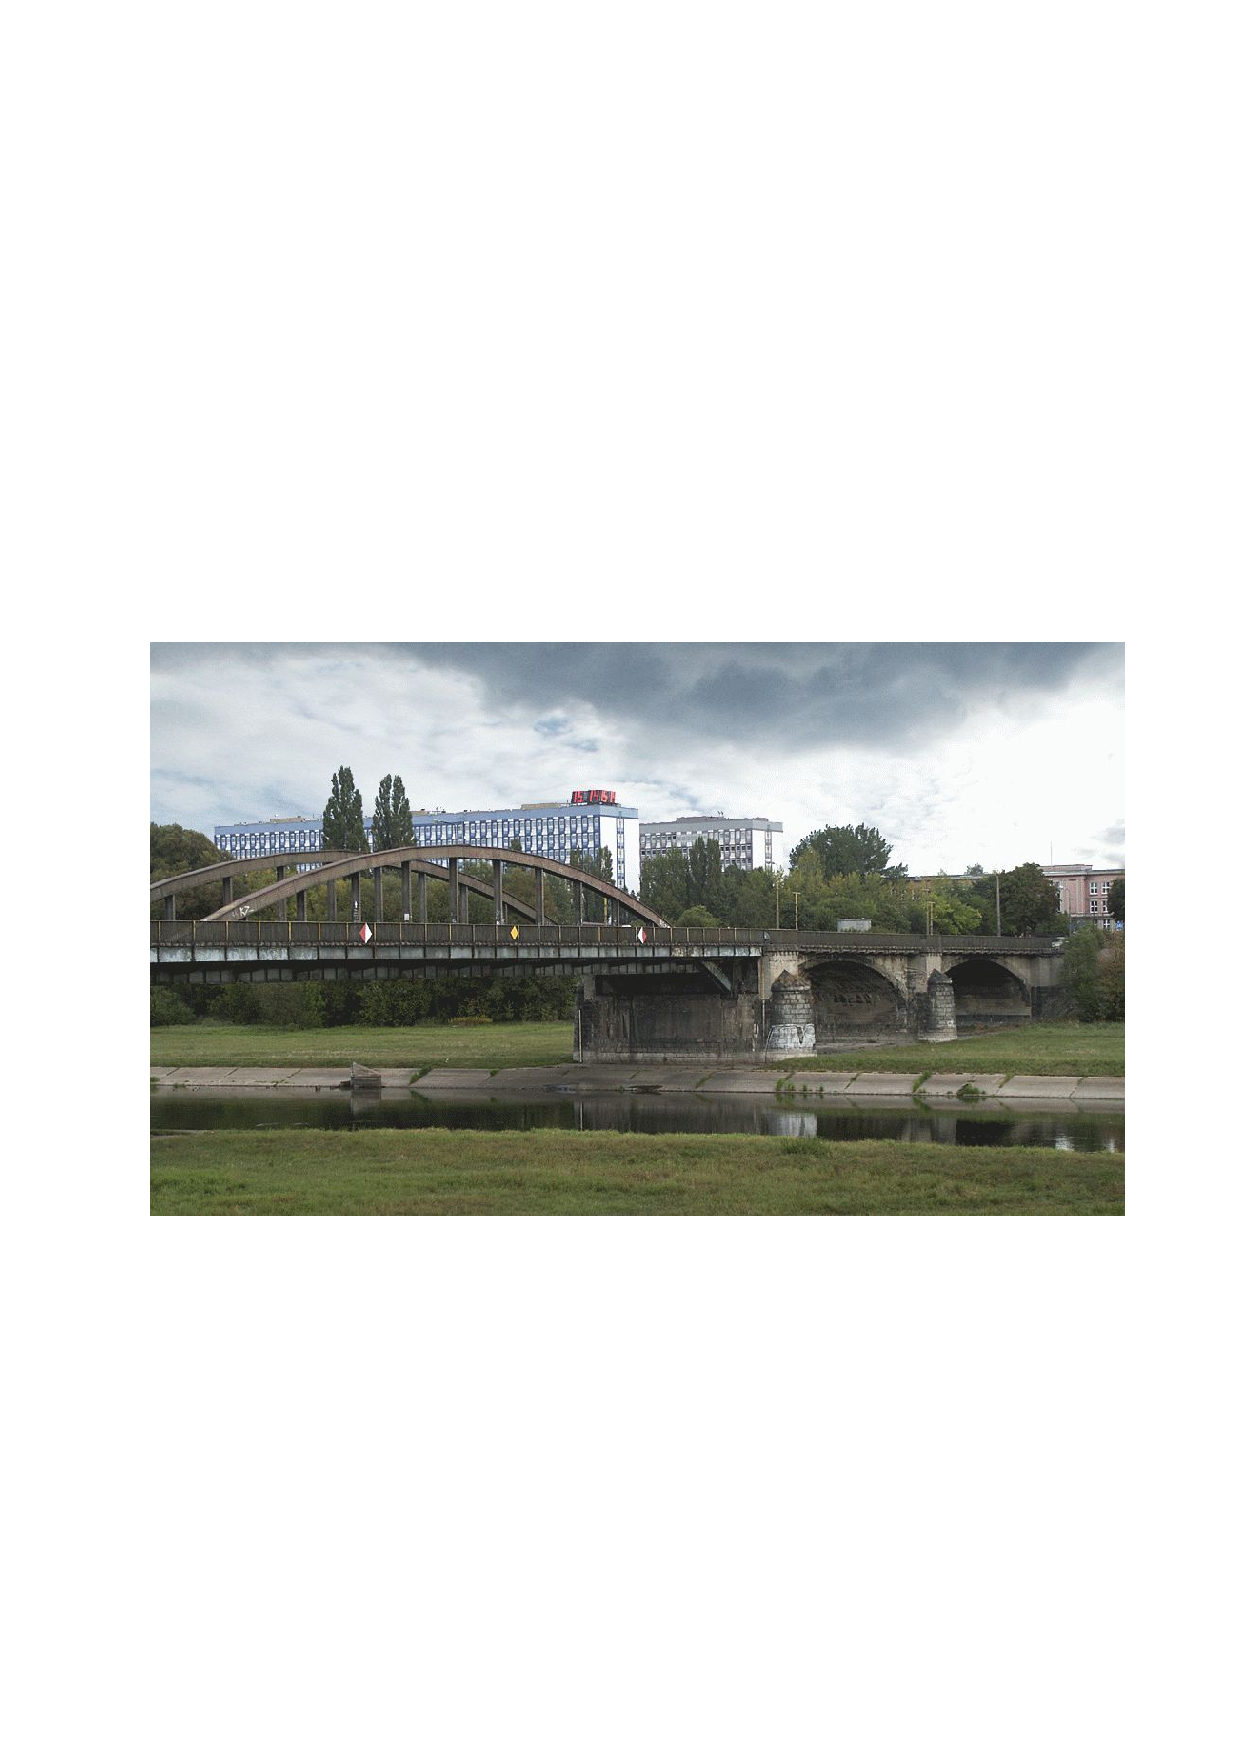
\includegraphics[width=8cm]{figures/cw-pp.jpg}
\end{center}
\caption{Budynki Instytutu Informatyki Politechniki Poznańskiej.}\label{rys:cwpp}
\end{figure}



\section{Wstawianie tablic}

Nowicjuszom polecam zrobienie tablic np.~w~Open Office i ich eksport do pliku
graficznego (lub PDF). Zaawansowani mogą spróbować wykonać je bezpośrednio
w \LaTeX{}u. Ważne jest, że nagłówki zwykle umieszcza się nad, a nie pod
obiektem (jak ma to miejsce w przypadku rysunków). Przykładowa tablica~\ref{tab:przyklad}
na stronie~\pageref{tab:przyklad} prezentuje jak to wygląda w kodzie.

\begin{table}
\caption{Przykład prostej tabeli.}\label{tab:przyklad}
\begin{center}
    \begin{tabular}{l | c}
    artykuł & cena [zł] \\
    \hline
    bułka   & $0.4$ \\
    masło   & $2.5$ \\
    \end{tabular}
\end{center}
\end{table}



\section{Bibliografia}

Polecam pakiet Bib\TeX, który ułatwia znakomicie zapis i spójne formatowanie
pozycji bibliograficznych. W kodzie źródłowym (plik \texttt{references.bib}) znajduje
się parę przykładów. Cytowanie z tekstu pracy uzyskujemy przy pomocy
polecenia \texttt{cite}. Przykładowo, Weiss i Stefanowski opisują system
Carrot$^2$ w pracy~\cite{stefanowski_weiss_awic2003}.



\subsection{Materiały instruktażowe}

Dokumentacji do systemu \LaTeX{} jest mnóstwo (zarówno w internecie, jak i~drukowanej).
Ten podręcznik wydaje się dobrym startem: \url{http://www.gust.org.pl/PDF/lshort2e.pdf}.





%
% Bibliografia i załączniki
%

\bibliographystyle{plplain}
{\small\bibliography{references}}

\backmatter


\chapter{XML Schema dla plików wejściowych i~wyjściowych}\label{schema}

W dodatku tym zostały zawarte specyfikacje formatów plików wejściowych i wyjściowych dla programu MultiSched.

\begin{listing}
\caption{XML Schema dla pliku opisującego dane wejściowe do algorytmu szeregowania zadań jednorodnych.}
\begin{codeblock}
<?xml version="1.0" encoding="utf-8" ?>
<xs:schema targetNamespace="http://tempuri.org/XMLSchema.xsd"  elementFormDefault="qualified"
xmlns="http://tempuri.org/XMLSchema.xsd" xmlns:mstns="http://tempuri.org/XMLSchema.xsd"
xmlns:xs="http://www.w3.org/2001/XMLSchema">
<xs:element name="schedule">
<xs:complexType>
<xs:sequence>
<xs:element name="dataVolumeSize" type="xs:unsignedLong" />
<xs:element name="numberOfTasks" type="xs:positiveInteger" />
<xs:element name="numberOfProcessors" type="xs:positiveInteger" />
<xs:element name="numberOfPacks" type="xs:positiveInteger" />
<xs:element name="processorsData">
<xs:complexType>
<xs:sequence>
<xs:element name="processor" maxOccurs="unbounded">
<xs:complexType>
<xs:attribute name="id" type="xs:ID" />
<xs:sequence>
<xs:element name="cost" type="xs:float" />
<xs:element name="processingRate" type="xs:float" />
<xs:element name="communicationRate" type="xs:float" />
<xs:element name="communicationStartupTime" type="xs:float" />
<xs:element name="bufferSize" type="xs:float" />
</xs:sequence>
</xs:complexType>
</xs:element>
</xs:sequence>
</xs:complexType>
</xs:element>
<xs:element name="geneticAlgorithmParameters" minOccurs="0">
<xs:complexType>
<xs:sequence>
<xs:element name="populationSize" type="xs:positiveInteger" />
<xs:element name="maxLengthOfIndividualsInStartPopulation" type="xs:positiveInteger" />
<xs:element name="mutationPercent" type="xs:decimal" />
<xs:element name="crossPercent" type="xs:decimal" />
<xs:element name="numberOfIterationsToStop" type="xs:positiveInteger" />
<xs:element name="numberOfIterationsWithoutImprovementToStop" type="xs:positiveInteger" />
<xs:element name="tournamentGroupSize"  type="xs:nonNegativeInteger" />
<xs:element name="startPopulationGenerationMethod">
<xs:simpleType>
<xs:restriction base="xs:nonNegativeInteger">
<xs:enumeration value="0" />
<xs:enumeration value="1" />
</xs:restriction>
</xs:simpleType>
</xs:element>
<xs:element name="minLengthOfIndividualsInStartPopulation" type="xs:positiveInteger" />
<xs:element name="selectionMethod">
<xs:simpleType>
<xs:restriction base="xs:positiveInteger">
<xs:enumeration value="1" />
<xs:enumeration value="2" />
</xs:restriction>
</xs:simpleType>
</xs:element>
<xs:element name="methodOfChoosingCrossPoint">
<xs:simpleType>
<xs:restriction base="xs:positiveInteger">
<xs:enumeration value="1" />
<xs:enumeration value="2" />
</xs:restriction>
</xs:simpleType>
</xs:element>
<xs:element name="methodOfMutation">
<xs:simpleType>
<xs:restriction base="xs:positiveInteger">
<xs:enumeration value="1" />
<xs:enumeration value="2" />
</xs:restriction>
</xs:simpleType>
</xs:element></xs:sequence></xs:complexType></xs:element>
</xs:sequence></xs:complexType></xs:element></xs:schema>
\end{codeblock}
\end{listing}

\begin{listing}
\caption{XML Schema dla pliku opisującego pluginy dostępne w systemie.}
\begin{codeblock}
<?xml version="1.0" encoding="utf-8" ?>
<xs:schema targetNamespace="http://tempuri.org/XMLSchema.xsd"
elementFormDefault="qualified"
xmlns="http://tempuri.org/XMLSchema.xsd"
xmlns:mstns="http://tempuri.org/XMLSchema.xsd"
xmlns:xs="http://www.w3.org/2001/XMLSchema">
<xs:element name="plugins">
<xs:complexType>
<xs:sequence>
<xs:element name="plugin" maxOccurs="unbounded">
<xs:complexType>
<xs:sequence>
<xs:element name="algorithm">
<xs:complexType>
<xs:sequence>
<xs:element name="name" type="xs:string" />
<xs:element name="author" type="xs:string" />
<xs:element name="description" type="xs:string" />
<xs:element name="type">
<xs:simpleType>
<xs:restriction base="xs:string">
<xs:enumeration value="exact" />
<xs:enumeration value="heuristic" />
</xs:restriction>
</xs:simpleType>
</xs:element>
<xs:element name="returnResults" type="xs:boolean" />
<xs:element name="bufferConstraints" type="xs:boolean" />
</xs:sequence>
</xs:complexType>
</xs:element>
<xs:element name="location" type="xs:string" />
</xs:sequence>
</xs:complexType>
</xs:element>
</xs:sequence>
</xs:complexType>
</xs:element>
</xs:schema>
\end{codeblock}
\end{listing}

\begin{listing}
\caption{XML Schema dla pliku opisującego znalezione uszeregowanie.}
\begin{codeblock}
<?xml version="1.0" encoding="utf-8" ?>
<xs:schema targetNamespace="http://tempuri.org/XMLSchema.xsd"
elementFormDefault="qualified"
xmlns="http://tempuri.org/XMLSchema.xsd"
xmlns:mstns="http://tempuri.org/XMLSchema.xsd"
xmlns:xs="http://www.w3.org/2001/XMLSchema">
<xs:element name="schedule">
<xs:complexType>
<xs:sequence>
<xs:element name="cmax" type="xs:double" />
<xs:element name="actions">
<xs:complexType>
<xs:sequence>
<xs:element name="action" maxOccurs="unbounded">
<xs:complexType>
<xs:sequence>
<xs:element name="packID" type="xs:positiveInteger" />
<xs:element name="packSize" type="xs:float" />
<xs:element name="processor" type="xs:positiveInteger" />
<xs:element name="direction">
<xs:simpleType>
<xs:restriction base="xs:string">
<xs:enumeration value="sending" />
<xs:enumeration value="receipt" />
</xs:restriction>
</xs:simpleType>
</xs:element>
</xs:sequence>
<xs:attribute name="id" type="xs:ID" />
</xs:complexType>
</xs:element>
</xs:sequence>
</xs:complexType>
</xs:element>
</xs:sequence>
</xs:complexType>
</xs:element>
</xs:schema>
\end{codeblock}
\end{listing}


%\normalfont
%\clearpage
%\input{symbols.tex}

%\clearpage
%\listoffigures

%\clearpage
%\listoftables

{\clearpage\footnotesize\printindex}


\end{document}
}

% other boxes
\def\boxbgcolor{white}
\def\boxfrcolor{blue!50}

% motivation box
\posterbox[Motivation]{16}{6}{8}{8.5}{\def\prc{\linewidth / 100}
\begin{textblock*}{\prc * 100}(0cm,0cm)%
\textbf{No diversity $\rightarrow$ no choice}
\begin{mylist}
\item no option for a DM: only one solution (the best one?)
\item the best solution is the magic one (w.r.t. one objective)
\end{mylist}

\textbf{Unrealistic assumptions}
\begin{mylist}
\item deterministic parameters, e.g. travel times, are unrealistic
\item stochastic models contain too strong assumptions
\end{mylist}
\end{textblock*}
}

% FVRPTW box
\posterfancybox[Fuzzy VRPTW]{0}{6}{15.5}{31}{\begin{textblock*}{\posterboxwidth}(0cm,0cm)

	\centering
	\textbf{Service start times}\\[.5em]

	\def\twindow{\draw (2,0) -- ++(0,1) -- ++(6,0) -- ++(2,-1);}

	% FUZZY ROUTE
	\def\xshift{12}
	\def\xfirstshift{-5}
	\FPeval{\xxshift}{clip(2*xshift)}
	\FPeval{\xxxshift}{clip(3*xshift)}
	\FPeval{\figwidth}{clip(-xfirstshift+3*xshift)}
	\begin{tikzpicture}[x=\posterboxwidth / \figwidth,y=\posterboxheight / 15,join=round]
	
	\draw[->] (\xfirstshift,0) -- +(\figwidth,0) node[below left] {$t$};
	
	\twindow
	\draw[red,very thick] (-4,0) -- ++(2,1) coordinate (A) -- ++(2,-1);
	\draw[red,loosely dotted] (A.base) -- +(0,-1);
	\draw[green,very thick] (2,0) -- +(0,1) -- +(0,0);
	\draw (-3.5,0) node[below right,inner sep=0pt] {\parbox{\posterboxwidth * \xshift / \figwidth}{\begin{mylist}
		\item arrival before time window
		\item service starts at the beginning of time window
	\end{mylist}}};
	\begin{scope}[shift={(\xshift,0)}]
	\twindow
	\draw[red,very thick] (1,0) -- ++(1,0.5);
	\draw[green,very thick] (2,0) -- ++(0,0.5) -- ++(1,0.5) coordinate (A) -- ++(2,-1);
	\draw[green,loosely dotted] (A.base) -- +(0,-1);
	\draw (-1.5,0) node[below right,inner sep=0pt] {\parbox{\posterboxwidth / \figwidth * \xshift}{\begin{mylist}
		\item arrival during allowed time window
		\item service start is ``clipped'' by the start of time window
	\end{mylist}}};
	\end{scope}
	
	\begin{scope}[shift={(\xxshift,0)}]
	\twindow
	\draw[green,very thick] (3,0) -- ++(2,1) coordinate (A) -- ++(2,-1);
	\draw[green,loosely dotted] (A.base) -- +(0,-1);
	\draw (0.5,0) node[below right,inner sep=0pt] {\parbox{\posterboxwidth / \figwidth * \xshift}{\begin{mylist}
		\item arrival during allowed time window
		\item service start = arrival time
	\end{mylist}}};
	\end{scope}
	\end{tikzpicture}
\end{textblock*}


\begin{textblock*}{\posterboxwidth / 100 * 55 - 2ex}(0cm,\posterboxheight /4 - 2em)
	\def\axis{
		\draw[->] (0,0) -- (3.8,0) node[below left] {$t$};
		\draw[->] (0,0) -- (0,1.5) node[below left] {$\mu(t)$};
	}


	% TIME WINDOWS
	\centering
	\textbf{Models of customer time window}\\[0.5em]
	
	\begin{tikzpicture}[x=\posterboxwidth / 2 / 5,y=\posterboxheight/2 / 7]
	\def\yshift{-2}
	\def\xdescdist{-0.8}
	\FPmul{\yyshift}{2}{\yshift}

	% fuzziness border
	\draw[loosely dotted] (3,0) -- (3,\yyshift);
	
	% crisp case
	\axis
	\draw (1,0) -- (1,1) -- (3,1) -- (3,0);
	\draw (2,1) node[above=2pt,font=\itshape,fill=white] { classical (``rigid'') };
	
	% fuzzy, tight case
	\begin{scope}[shift={(0,\yshift)}]
		\axis
		\draw (1,0) -- (1,1) -- (2.5,1) -- (3,0);
		\draw (2,1) node[above=2pt,font=\itshape,fill=white] { important (``tight'') };
	\end{scope}
	
	% fuzzy, loose case
	\begin{scope}[shift={(0,\yyshift)}]
		\axis
		\draw (1,0) -- (1,1) -- (3,1) -- (3.5,0);
		\draw (2,1) node[above=2pt,font=\itshape,fill=white] { less important (``loose'') };
	\end{scope}
	
	% side notes: cirsp and fuzzy
	\FPadd\yboxlen{-\yshift}{1.5}
	\FPeval\ytextpos{yshift * 2/3 - 0.75}
	\draw[snake=brace, very thick, segment amplitude=.5em] (\xdescdist,0) -- +(0,1.5);
	\draw[snake=brace, very thick, segment amplitude=.5em] (\xdescdist,\yyshift) -- +(0,\yboxlen);
	
	\FPadd{\xxdescdist}{\xdescdist}{-0.1}
	\draw (\xxdescdist,0.75) node[above,rotate=90] {crisp model};
	\draw (\xxdescdist,\ytextpos) node[above,rotate=90] {fuzzy model};
	
	\end{tikzpicture}\\[2em]
	
	
	% TRAVEL TIMES
	\textbf{Intuitive uncertain travel times}\\[0.5em]
	
	\begin{tikzpicture}[x=\posterboxwidth/3 / 5,y=\posterboxheight/2 / 7]
	
	\axis
	\draw (0.5,0) node[below] {\vphantom{b}a} -- (1,1) -- (2,0) node[below] {\vphantom{b}c};
	\draw[dotted] (1,0) node[below] {b} -- +(0,1);
	
	\draw (1.3,1.5) node[below right] {\parbox{\posterboxwidth / 3}{\raggedleft\itshape The travel is most
		likely to take \textrm{b}, although it can last as long as \textrm{c};
		however, sometimes \textrm{a} is enough.}};
	\end{tikzpicture}\\[2em]
	
	\parbox{\posterboxwidth/3 * 13 / 10 + 2em}{The problem contains two objectives:
	\begin{mylist}
		\item maximization of satisfaction
		\item minimization of cost
	\end{mylist}}
\end{textblock*}
}{%
(0,0) -- (0pt,31\TPVertModule) -- (15.5\TPHorizModule,31\TPVertModule) -- (15.5\TPHorizModule,22.5\TPVertModule) -- (8.5\TPHorizModule,22.5\TPVertModule) -- (8.5\TPHorizModule,0pt) -- cycle;
}

% PMA box
\posterfancybox[Pareto Memetic Algorithm]{24.5}{6}{15.5}{31}{\begin{textblock*}{\posterboxwidth}(0cm,0cm)
\centering%
\textbf{Main loop of the multiobjective evolutionary algorithm}\\[.5em]

\def\figscale{.5}
\def\figfontsize{\footnotesize}

\newcommand\pmabox[1]{%
\scalebox{\figscale}{%
\begin{tikzpicture}[font=\figfontsize]
\input{vector/StagesPMA_#1}
\draw (7,1.5) node[font=\normalsize,draw,circle] {#1};
\end{tikzpicture}}%
}

\newcommand\circled[1]{%
\raisebox{-.5em}{\tikz \draw (0,0) node[circle,draw] {#1};}%
}

\begin{tabular}{ccc}
\hspace{1em}\parbox[b]{4cm}{%
\small%
1. Choose a direction\\
2. Choose parents\\
3. Recombine\\
4. Do local search\\
5. Update Pareto set\\
\vspace*{1.5ex}
}&\pmabox{1}&\pmabox{2}\\
\pmabox{3}&\pmabox{4}&\pmabox{5}
\end{tabular}
\end{textblock*}

\begin{textblock*}{\posterboxwidth / 100 * 55 - 2ex}(\posterboxwidth / 100 * 45 + 2ex,\posterboxheight /4)
\centering%
\textbf{Achievement scalarizing functions}\\[.5em]

\scalebox{.5}{%
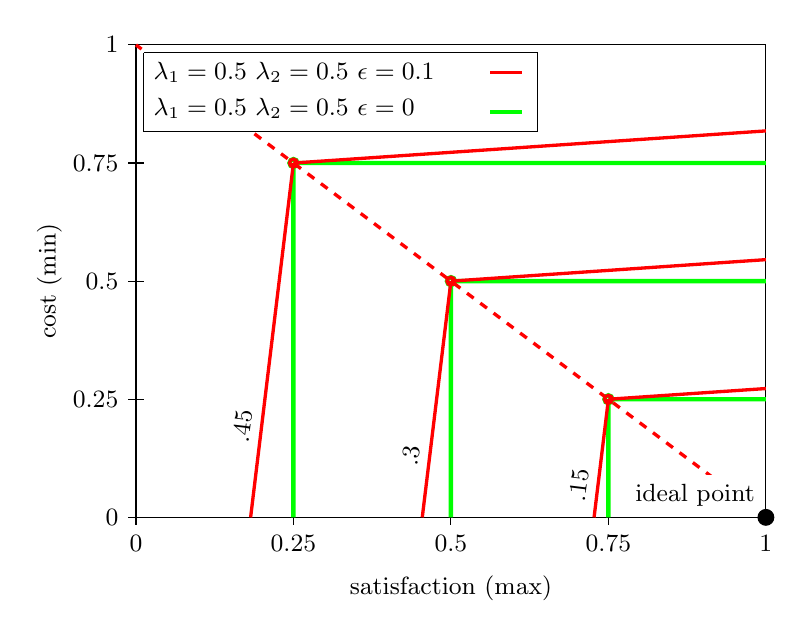
\begin{tikzpicture}[font=\small]
	% The axes
	\draw (0, 0) -- (8, 0) -- (8, 6) -- (0, 6) -- (0, 0);
	% Description of the axes
	\draw (4, -0.9) node[anchor=center] {satisfaction (max)};
	\draw [rotate=90] (3, +1.1) node[anchor=center, rotate=90] {cost (min)};
	% Ticks on the horizontal axis
	\foreach \x / \xtext in {0 / 0, 2 / 0.25, 4 / 0.5, 6 / 0.75, 8 / 1}
		\draw (\x cm, 0.1cm) -- (\x cm, -0.1cm) node[anchor=north]{\xtext};
	% Ticks on the vertical axis
	\foreach \y / \ytext in {0 / 0, 1.5/ 0.25, 3 / 0.5, 4.5 / 0.75, 6 / 1}
		\draw (-0.1cm, \y cm) node[anchor=east]{\ytext} -- (0.1cm, \y cm);
	% The related Tchebycheff weighted scalarizing function
	\begin{scope}[ultra thick, green]
	\draw (6, 0) -- node[near start, above, sloped, black]{} (6, 1.5) ++(0, 0) circle (0.05cm) -- (8, 1.5);
	\draw (4, 0) -- node[near start, above, sloped, black]{} (4, 3) ++(0, 0) circle (0.05cm) -- (8, 3);
	\draw (2, 0) -- node[near start, above, sloped, black]{} (2, 4.5) ++(0, 0) circle (0.05cm) -- (8, 4.5);
	\end{scope}
	% The achievement weighted scalarizing function
	\begin{scope}[very thick, red]
	\draw (5.818, 0) -- node[near start, above, sloped, black]{.15} (6, 1.5) ++(0, 0) circle (0.05cm) -- (8, 1.636);
	\draw (3.636, 0) -- node[near start, above, sloped, black]{.3} (4, 3) ++(0, 0) circle (0.05cm) -- (8, 3.273);
	\draw (1.456, 0) -- node[near start, above, sloped, black]{.45} (2, 4.5) ++(0, 0) circle (0.05cm) -- (8, 4.908);
		% the line through vertices
	\draw[dashed] (8, 0) -- (0, 6);
	\end{scope}
	% Legend
	\filldraw[fill=white,draw=black] (0.1, 5.9) -- (5.1, 5.9) -- (5.1, 4.9) -- (0.1, 4.9) -- (0.1, 5.9); % the boundary
	\draw (0.1, 5.9) node[anchor=north west] {$\lambda_1=0.5\ \lambda_2=0.5\ \epsilon=0.1$}; % first function text
	\draw[very thick, red] (4.5, 5.65) -- ++(0.4, 0); % first function line
	\draw (0.1, 5.45) node[anchor=north west] {$\lambda_1=0.5\ \lambda_2=0.5\ \epsilon=0$}; % second function text
	\draw[ultra thick, green] (4.5, 5.15) -- ++(0.4, 0); % second function line
	% The ideal point
	\draw (8, 0) node [above left=.5pt, fill=white] {ideal point};
	\filldraw[fill=black] (8, 0) circle (0.1cm);

\end{tikzpicture}}\\[1em]

\textbf{Local search: exchange of two customers}\\
\includegraphics[width=\posterboxwidth / 100 * 55 - 5ex]{bitmap/customerExchangeExample}\\[1em]

\textbf{Local search: relocation of a customer}\\
\includegraphics[width=\posterboxwidth / 100 * 55 - 5ex]{bitmap/customerRelocateExample}\\[1em]

\textbf{Route-based crossover}\\
\includegraphics[width=\posterboxwidth / 100 * 55 - 5ex]{bitmap/CEPXExample}\\[1em]

\textbf{Common edges preserving crossover}\\
\includegraphics[width=\posterboxwidth / 100 * 55 - 5ex]{bitmap/RBXExample}\\[1em]
\end{textblock*}}{%
(7\TPHorizModule,0pt) -- (7\TPHorizModule,22.5\TPVertModule) -- (0pt,22.5\TPVertModule) -- (0pt,31\TPVertModule) -- (15.5\TPHorizModule,31\TPVertModule) -- (15.5\TPHorizModule,0pt) -- cycle;
}

% additional conclusions box
\posterbox[Additional conclusions]{0}{37.5}{40}{10}{\begin{textblock*}{\posterboxwidth / 5}(0cm,0cm)

\def\figscale{.6}
\def\figfontsize{\small}

\newcommand\tikzbox[1]{%
\scalebox{\figscale}{%
\begin{tikzpicture}[font=\figfontsize]
\input{#1}
\end{tikzpicture}}%
}

\centering%
\textbf{Comparison of approximations: coverage C}\\[.5em]

\tikzbox{vector/QualityMeasures_C1}\\
\tikzbox{vector/QualityMeasures_C2}

\end{textblock*}


\begin{textblock*}{\posterboxwidth / 5}(\posterboxwidth * 4 / 5,0cm)

\def\figscale{.6}
\def\figfontsize{\small}

\newcommand\tikzbox[1]{%
\scalebox{\figscale}{%
\begin{tikzpicture}[font=\figfontsize]
\input{#1}
\end{tikzpicture}}%
}

\centering%
\textbf{Comparison of approximations: R measure}\\[.5em]

\tikzbox{vector/QualityMeasures_R1}\\
\tikzbox{vector/QualityMeasures_R2}

\end{textblock*}


\begin{textblock*}{\posterboxwidth * 3 / 5}(\posterboxwidth / 5,-0.7cm)%
\centering%
\begin{tabular}{lll}
\includegraphics[height=\posterboxheight * 6/10]{vector/Comparison_C}&\hspace{2em}&%
\includegraphics[height=\posterboxheight * 6/10]{vector/Comparison_R}\\
\hspace{1em}\parbox[t]{\posterboxwidth / 4}{%
	Comparison of instances:
	\begin{mylist}
	\item clustered instances are easier than random ones
	\item wide time window $\rightarrow$ easier random instances
	\item wide time window $\rightarrow$ harder clustered instances
	\end{mylist}%
}& &% 
\hspace{1em}\parbox[t]{\posterboxwidth / 4}{%
	Comparison of crossovers:
	\begin{mylist}
	\item RBX is random, CEPX is deterministic
	\item RBX is usually better than CEPX
	\item randomness in RBX is useful
	\end{mylist}%
}
\end{tabular}
\end{textblock*}
}

% enable grid mode (under the text)
%\begin{textblock*}{0cm}(\XMargin,\YMargin)\showgrid\end{textblock*}

% background last
\begin{textblock*}{\XMargin + 40\TPHorizModule + \XMargin}(0pt,0pt)%

\begin{tikzpicture}
	\fill[yellow!10] (0,0) rectangle (\XMargin + 40\TPHorizModule + \XMargin, \YMargin + 48\TPVertModule + \YMargin);
	\draw[thin] (0,0) rectangle +(\XMargin + 40\TPHorizModule + \XMargin, \YMargin + 48\TPVertModule + \YMargin);
\end{tikzpicture}
\end{textblock*}

\end{document}
